\documentclass{standalone}
\usepackage{chez}

\begin{document}
\chapter{September 02, 2020}
The first half of the course is on \vocab{homology}, where we want to study
space by asking how many ``holes'' a space has.

For example, a circle, the letter Y, and a line segment with
three circles attached to it have \(1\), \(0\), and \(3\) holes respectively.
\begin{center}
  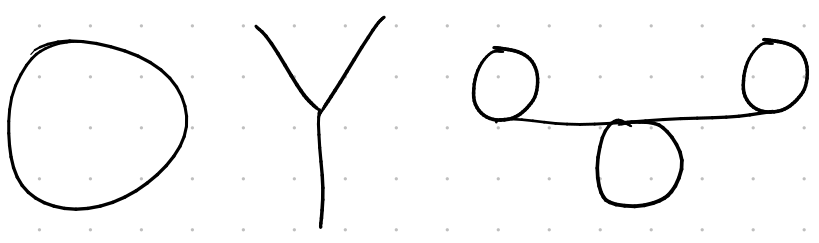
\includegraphics[width=0.5\textwidth]{18_905-200902-1.png}
\end{center}
The fundamental group is one way of measuring the number of holes, but we will
present a different way of understanding the number of holes in these spaces
with the first homology group \(H_1\).

Let's first provide an algorithm of how to find the homology of a space.
\begin{example}[Homology of the circle]
  First, we transform the space into a more graph-theoretic structure
  by adding some vertices, and then making the edges directed, like so:
  \begin{center}
    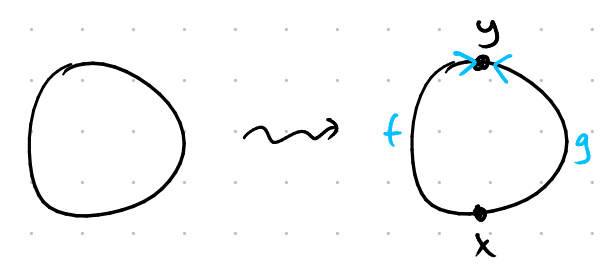
\includegraphics[width=0.5\textwidth]{18_905-200902-2.png}
  \end{center}
  Let \(\ZZ\{f, g\}\) denote the free abelian group generated by
  \(f\) and \(g\). Consider the group homomorphism
  \begin{align*}
    \partial \colon &\ZZ\{f, g\} \to \ZZ\{x, y\} \\
      & f \mapsto y - x \\
      & g \mapsto y - x,
  \end{align*}
  where we mapped each edge to their ``target minus source''. Note that
  the kernel of \(\partial\) is the integer multiples of \(f - g\).
  In particular, \(\ker \partial\) is generated by \emph{one} element,
  so there is \emph{one} hole.
  This kernel is called the first homology group \(H_1\) of the circle.
\end{example}

\begin{example}[Homology of the letter Y]
  Again, transform the space into a combinatorial gadget by assigning
  vertices and directing edges:
  \begin{center}
    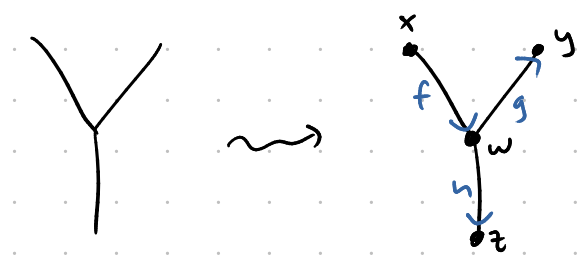
\includegraphics[width=0.5\textwidth]{18_905-200902-3.png}
  \end{center}
  We consider the homomorphism
  \begin{align*}
    \partial \colon & \ZZ\{f, g, h\} \to \ZZ\{x, y, z, w\} \\
      & f \mapsto w - x \\
      & g \mapsto y - w \\
      & h \mapsto z - w.
  \end{align*}
  The only element that gets sent to \(0\) by \(\partial\) is \(0\),
  so \(\ker \partial\) is the free abelian group on \(\nullset\).
  Therefore, there are no holes.
\end{example}

The kernel we have been computing is the first homology group,
and the number of generators corresponds to the number of holes.

This algorithm involves many arbitrary decisions.
  Why is it giving the same answer each time?
  How does this generalize to larger dimensional spaces?

\end{document}
